%!TEX root = ../physical-olympics-2.tex
\chapter{麦克斯韦方程组}


\section{麦克斯韦方程组}

\subsection{位移电流假说}

磁荷不存在,\,为电磁学规律带来了充分的简化.\,但是目前我们发现的三种现象:\,静止电荷产生电场,\,稳恒电流产生磁场,\,变化电流(通过产生变化的磁场)产生涡旋电场,\,并不是电磁学客观规律的全部.\,前两章我们已经充分说明,\,后两种现象其实都是相对性原理的后果:\,在一个参考系内不变的电荷分布,\,必将在另一个参考系看来产生电流,\,稳恒电流也会因为在另一个参考系而随时间变化,\,从而在一个参考系中纯粹的电场可以在另一个参考系内引发磁场和涡旋电场.\,电磁学的最后一种现象,\,由\emph{麦克斯韦}(J. C. Maxwell)在1861提出的,\,位移电流产生磁场的现象,\,在某种程度上也由相对性原理引发.\,我们之后就可以发现这一点.

\begin{wrapfigure}[15]{o}[-10pt]{6cm}
\vspace{-0.1cm}
\centering
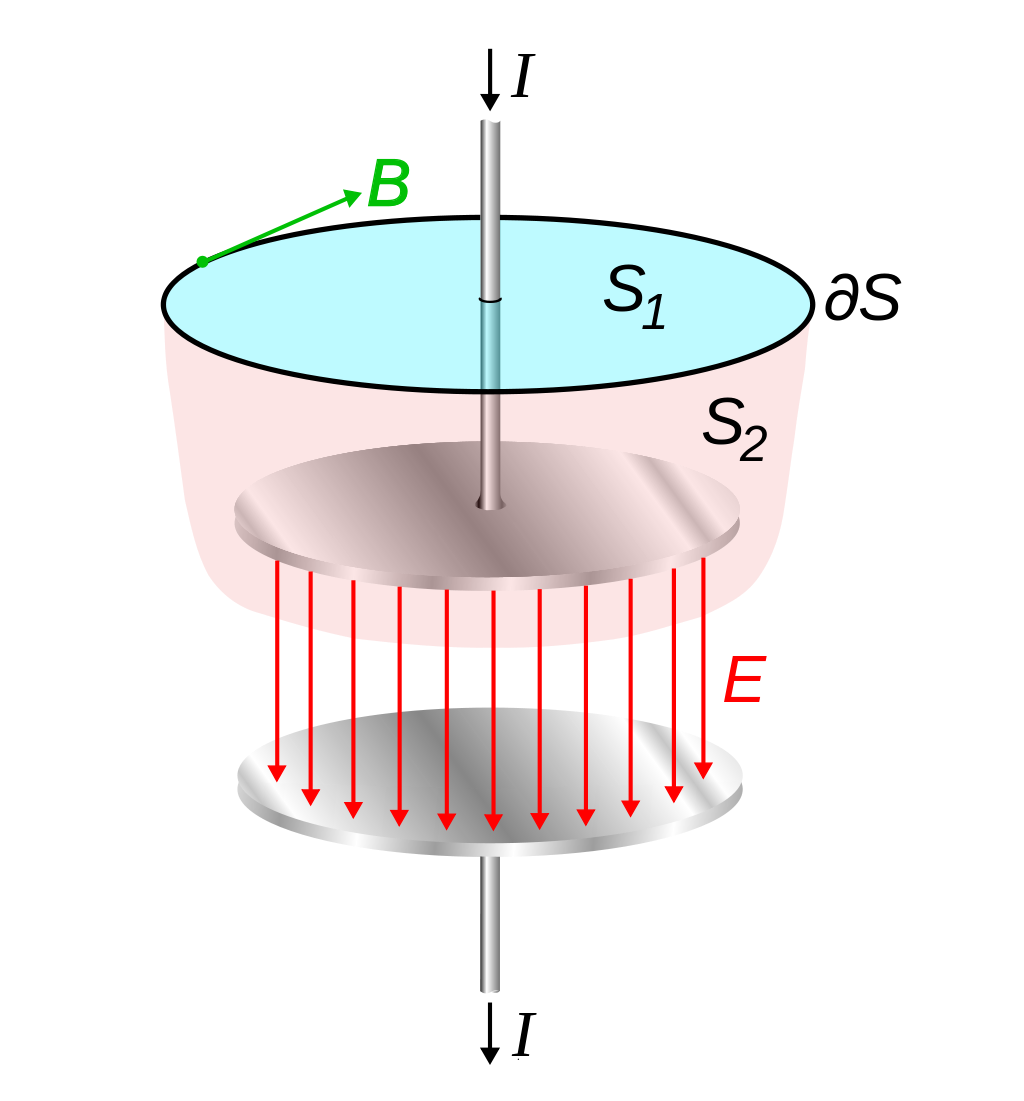
\includegraphics[width=6cm]{image/7-6-1.png}
\caption{修正安培环路定律}
\end{wrapfigure}
一切的源起,\,在于麦克斯韦对安培环路定律普遍性的质疑.\,我们不能认为在变化的荷与场的情况下,\,磁场的安培环路定律具有普适性.\,它写作:
\[\oint\limits_{\partial S} \bs{B}\cdot \ud \bs{l}{\color{red}{=}}\mu_0\int\limits_{S}\bs{j}\cdot \ud \bs{S}\]

为何质疑?\,考虑一个电容器不断充电的过程,\,如图所示.\,我们可以认为在距离电容较远的某点处,\,取一个垂直于导线的半径足够小的圆盘$S_1$后,\,边界环路上的磁场与导线上的电流之间符合安培环路定律的关系.\,但是注意到如果我们选择一个兜状的面$S_2$时,\,它的边界可以与圆盘边界完全一致.\,但是由于它把导线和一个极板完全兜住,\,故这个面上完全没有电流.\,从而就不能认为这个面和它的边界符合安培环路定律!\,至少,\,$S_1$和$S_2$绝对不可能同时符合安培环路定律!\,这是因为,\,等号左侧这两个面边界上具有同一个磁场的环路积分,\,但是等号右侧却是不一样的电流通量:\,$S_1$上为导线电流$I$而$S_2$上为零.\,两个等式是不可能同时成立的.

但是空间中的磁场又的确是客观存在的,\,而不是虚无缥缈的辅助物理量,\,我们依然可以通过对带电粒子受到的洛伦兹力的要求来确定空间中某处的磁场值:
\[\bs{F}=q(\bs{E}+\bs{v}\times\bs{B})\]

那么如何寻找这种情况下正确反映磁场计算方法的公式?\,麦克斯韦做到了这一点,\,而他的做法其实可以被简单的归纳为三点:

逻辑上要求自恰,\,数学上发展工具,\,哲学上遵从\emph{吝啬原则}(law of parsimony)\footnote{又做奥卡姆剃刀(Occam's razor):\, 如无必要,\,勿增实体.\,认为基本规律的不同表述之间越简单的描述约能反应基本规律的本质.}.

首先第一点,\,安培环路定律从逻辑上已经不能自洽了,\,所以必须修改它,\,一个合理的想法是为它增添一项:
\[\oint\limits_{\partial S} \bs{B}\cdot \ud \bs{l}=\mu_0\int\limits_{S}\bs{j}\cdot \ud \bs{S}+(?)\]

增添这一项的目的就是为了能避免如之前电容器充电情况下的矛盾情况的发生.\,事实上电容器充电的例子就提供了修改之后的表达式是否正确的试金石.

为了找到这个项,\,矢量微分工具就发挥了不可替代的作用.\,使用微分形式以上积分等式写作:
\[\nabla\times\bs{B}=\mu_0\bs{j}+(?)\]

再两边同时取散度,\,左边数学上一定变成零,\,从而得到添加的项需要符合的条件:
\[\mu_0\nabla\cdot \bs{j}+\nabla\cdot(?)=0\]

再注意到电荷电流符合连续性方程:
\[\nabla\cdot \bs{j}+\frac{\partial \rho}{\partial t}=0\]

从而得到:
\[\nabla \cdot (?)=\mu_0\frac{\partial \rho}{\partial t} \]

为了实现这一点,\,最简单的一种可能性为:
\[(?)=\mu_0\varepsilon_0\frac{\partial \bs{E}}{\partial t}\]

这是因为电场的散度就会回到电荷:
\[\nabla\cdot\bs{E}=\frac{\rho}{\varepsilon_0} \quad \Rightarrow \quad \nabla \cdot \left(\mu_0\varepsilon_0\frac{\partial \bs{E}}{\partial t}\right)=\mu_0\varepsilon_0\frac{\partial }{\partial t}(\nabla\cdot\bs{E})=\mu_0\frac{\partial \rho}{\partial t}\]

但是我们注意到,\,使得之前的要求成立的添加项$(?)$不是唯一的,\,事实上在刚刚的结果上添加任意一个矢量场的旋度都不改变其散度的值:
\[\nabla\cdot\left(\mu_0\varepsilon_0\frac{\partial \bs{E}}{\partial t}+\nabla\times \bs{F}\right)=\mu_0\frac{\partial \rho}{\partial t}+0\]

于是最后一个思想就发挥了作用:\,如无必要,\,勿增实体.\,往往简单而自洽的形式就能反映真实的物理规律.\,从而麦克斯韦就利用这样的推理得到了修正的安培环路定律:
\[\nabla\times\bs{B}=\mu_0\bs{j}+\mu_0\varepsilon_0\frac{\partial \bs{E}}{\partial t}\]

同时麦克斯韦提出了以下视角去解释以上式子背后的物理图像:\,我们定义\emph{位移电流}(displacement current):
\[\bs{j}_d=\varepsilon_0\frac{\partial \bs{E}}{\partial t}\]

那么我们的工作可以归纳为一句话:\,通过引入虚构位移电流,\,导致与真实电流的和形成一个没有散度(即连续)的电流场:
\[\nabla\cdot(\bs{j}+\bs{j}_d)=0\]

举例来说,\,在之前的电容器充电的场合下,\,如果忽略电容器的边缘效应,\,那么从上方往下通过的电流为$I$时,\,电容器上积累的面电荷密度$\sigma$的增长为:
\[I=\dot{\sigma}S\]

从而电容内部的场强就会随之增长:
\[E=\frac{\sigma}{\varepsilon_0}\quad \Rightarrow \quad \dot{E}=\frac{I}{\varepsilon_0S}\]

从而把电场的导数视作位移电流的话,\,造成的总电流就是:
\[I_d=j_d S=\varepsilon_0 \dot{E} S=I\]

从而实际上补充位移电流后电流并没有在电容器极板上中断,\,这样也就不会造成之前电容器上不同面上电流不同而造成的矛盾情况.

如果认为补充这一项后形成的新安培环路定律具有在任意变化的电磁场下的普适性,\,我们可以发现,\,这样的一条规律在数学形式上具有与感生电场规律具有某种``对称性''.\,尤其是当空间中某处没有通过实际电流时,\,此时两条规律分别为:
\[\nabla\times \bs{E}=-\frac{\partial \bs{B}}{\partial t}\]
\[\nabla\times\bs{B}=\mu_0\varepsilon_0\frac{\partial \bs{E}}{\partial t}\]

即,\,变化的磁场(部分来源于变化的电流分布)会产生电场,\,变化的电场(部分来源于变化的电荷分布)会产生磁场.

我们曾经解释过第一个式子,\,它实际上可以解释为动生电动势现象的相对论效应.\,即在一个参考系中的磁场会在另一个参考系中招致电场:
\[\bs{E}'=\bs{v}\times \bs{B}\]

而一个参考系中的电场在另一个参考系中招致磁场这样的对称行为,\,实际上我们在之前静磁学章节中建立毕奥-萨伐尔定律时就已经有介绍过,\,得到的结果为:
\[\bs{B}'=-\frac{\bs{v}\times \bs{E}}{c^2}\]

这就不难看出两者之间的对称性来.\,而第一个式子,\,我们通过一个参考系中的动生电动势与另一个参考系中的感生电动势都与法拉第电磁感应定律相联系的思路,\,就推出了电场的旋度公式:
\[\bs{E}'=\bs{v}\times \bs{B}\quad \Rightarrow\quad  \oint\limits_{\partial S} \bs{E}\cdot \ud \bs{l}=-\int\limits_S \frac{\partial \bs{B}}{\partial t}\cdot \ud\bs{S}\quad \Rightarrow \quad  \nabla\times \bs{E}=-\frac{\partial \bs{B}}{\partial t}\]

注意到系数$1/c^2$实际上就是$\mu_0\varepsilon_0$,\,完全仿照这个过程,\,我们也能得到磁场的环量也将等于电通量的导数,\,即对应有:
\[\bs{B}'=-\frac{\bs{v}\times \bs{E}}{c^2}\quad \Rightarrow\quad  \oint\limits_{\partial S} \bs{B}\cdot \ud \bs{l}=\mu_0\varepsilon_0\int\limits_S \frac{\partial \bs{E}}{\partial t}\cdot \ud\bs{S}\quad \Rightarrow \quad  \nabla\times \bs{B}=\mu_0\varepsilon_0\frac{\partial \bs{E}}{\partial t}\]

所以至此我们可以总结:\,电磁学的所有规律,\,都可以看做唯一一个规律:\,即库仑定律,\,在相对论原理下分化出来的丰富变式.


\subsection{麦克斯韦方程组}

将四个规律:\,电荷产生电场,\,电流产生磁场,\,变化的磁场产生电场,\,变化的电场产生磁场组合到一起,\,就得到了\emph{麦克斯韦方程}(Maxwell equations),\,实际上指以下方程组\footnote{但是其实这四个方程是一个整体,\,正如电磁场本身应当视作一个整体对待}:
\begin{align*}
\nabla\cdot \bs{E} &=  \frac{\rho }{\varepsilon_0}\\
\nabla\times \bs{E} &=   -\frac{\partial \bs{B}}{\partial t} \\
\nabla\cdot \bs{B} &=  0 \\
\nabla\times\bs{B} &=\mu_0\bs{j}  +  \varepsilon_0\mu_0\frac{\partial \bs{E}}{\partial t}
\end{align*}

它完整而全面地描述了场与荷之间的关系.\,在之前的观点中,\,我们认为电荷是因,\,场是结果.\,这种观点之后将不再适用,\,这是因为在数学形式上,\,变化的电场和磁场可以互相产生,\,之后我们利用这一点能找到完全脱离电荷存在的电磁波解.\,而完整的电磁理论实际上只需要再配合电场磁场本身的定义,\,即洛伦兹的力公式:
\[\bs{F}=q(\bs{E}+\bs{v}\times \bs{B})\]

然而,\,同样的一个现象(电荷与场之间的相互作用)可以有不同理论来描述.\,力学我们就曾经介绍过牛顿经典力学体系和尝试过分析力学的可能性.\,静电学和静磁学中,\,电场和磁场不仅可以由场强来描述,\,我们也研究了由势来描述的可能性.\,当时的势与电荷的关系是比较简单的:
\[\varphi=\int\ke \frac{\rho}{r}\ud V \quad ,\quad \bs{A}=\int \kb \frac{\bs{j}}{r}\ud V\]

那么能不能为变化的电磁场整体采取一个用势来描述的方法?\,至少以上两个式子应当被摒弃,\,因为他们只描述了电荷直接产生的电场与电流直接产生的磁场.\,而我们知道变化的电荷与电流可以交叉地产生磁场和电场.\,事实上之前成立的以下两个描述势与场强之间关系的式子也应当考虑摒弃:
\[\bs{E}=-\nabla \varphi\quad,\quad \bs{B}=\nabla \times \bs{A} \]

后一个式子不会招致明显的矛盾,\,因为即使在变化电磁场下,\,依然有:
\[\nabla\cdot \bs{B}=0\]

故无需添加新项即可成为恒等式.

矛盾集中体现在第一条上.\,两边同时取旋度就能看出其中的不妥之处:
\[\nabla \times \bs{E}=-\nabla \times\nabla \varphi\]

其中左侧根据麦克斯韦方程,\,它等于磁场的对时间变化率,\,它不需要为零.\,但是右侧根据数学规律它必然为零.\,这就造成了矛盾.

解决这个问题的核心思想,\,其实与麦克斯韦发现位移电流的思想完全一致.\,我们添加一个项以使得矛盾消除,\,以相同的思路推理,\,过程留给读者,\,可得这个项为:
\[\bs{E}=-\nabla \varphi-\frac{\partial \bs{A}}{\partial t}\]

这一点本身又不难理解.\,我们知道完整的电磁理论有四个要素,\,在最低阶的近似下之前的式子反映了电荷直接产生电场与电流直接产生磁场的要素.\,那么我们添加的项实际上反映了变化的电流产生电场的要素:\,因为磁矢势由电流产生,\,那么它的导数自然反映了变化的电流,\,而它构成了电场的第二项.

而变化的电荷产生磁场,\,它不会在新的场与势的关系式中体现,\,这是因为这样的改变直接同时改变了$\bs{B}$和$\bs{A}$的值.\,前者通过位移电流,\,后者之后介绍.\,从而使得$\bs{B}=\nabla \times \bs{A}$依然成立.\,从而我们总结出任意情况下描述电磁场的标势和矢势需要符合的关系:
\[\bs{E}=-\nabla \varphi-\frac{\partial \bs{A}}{\partial t}\quad ,\quad\bs{B}=\nabla \times \bs{A}\]

但是,\,接下来我们会引入一个惊人的不确定性:\,其中的端倪在静电静磁学中其实已经出现苗头:\,电势,\,具有一个整体常数的不确定性,\,这是因为电势的零点选取其实本质上是任意的,\,以下变换后产生的标量场依然可以作为电势:
\[\varphi'(\bs{r})=\varphi(\bs{r})+C\]

只有进一步规定无穷远处的电势为零才能回到之前点电荷积分的电势公式:
\[\varphi(\infty)=0\]

而静磁场的情况则更具有戏剧性:\,我们之前通过电流元直接积分产生的磁矢势其实符合以下性质:
\[\nabla\cdot\bs{A}=0\]

当然以上两个结果都还要求势不随时间改变,\,比如:
\[\frac{\partial \varphi}{\partial t}=0\]

如果仅仅希望能通过磁矢势的旋度计算磁场$\nabla\times \bs{A}=\bs{B}$,\,即使进一步要求$\nabla\cdot\bs{A}=0$,\,$\bs{A}$的取法其实也不唯一.\,可以证明,\,如果找到所谓的三维调和函数,\,即在全空间满足以下规律的标量场:
\[\nabla^2\phi=0\]

常数就属于调和函数,\,除此之外我们还能举出很多的例子:
\[\phi=x\;,\;x^2-y^2\;,\;xy\;,\;x^2+y^2-2z^2\;,\;e^{x}\sin y\;,\;\cdots\]

那么任意找一个调和函数梯度形成的矢量场:
\[\bs{F}=\nabla\phi\]

那么不难看出这个场就会符合:
\[\nabla\times\bs{F}=\bs{0}\quad ,\quad \nabla \cdot \bs{F}=0 \]

从而以下对磁矢势的变换就可以在不改变对磁矢势的要求下,\,造成同一个磁场:
\[\bs{A}'=\bs{A}+\bs{F}\]
\[\nabla\cdot\bs{A}'=\nabla\cdot\bs{A} =0\quad \&\quad \nabla \times \bs{A}'=\nabla\times \bs{A} =\bs{B}\]

我们从其中归纳出两个概念.\,一是我们要求电势和矢势根据具体问题不同选取不同的条件,\,上面过程中出现的各种要求就有:
\[\nabla\cdot\bs{A}=0\]
\[\frac{\partial \varphi}{\partial t}=0\]
\[\varphi(\infty)=0\]

这些称作\emph{规范条件}(gauge condition).\,或者简单称作\emph{规范}.

但是,\,即使存在规范条件,\,例如静磁场下要求$\nabla\cdot\bs{A}=0$,\,或者进一步放宽干脆没有任何规范条件的限制,\,我们发现电势和矢势其实不是位移确定的,\,同样的一个电磁场,\,在下式成立的条件下:
\[\bs{E}=-\nabla \varphi-\frac{\partial \bs{A}}{\partial t}\quad ,\quad\bs{B}=\nabla \times \bs{A}\]

势$\varphi,\,\bs{A}$存在不同的取法,\,普遍来说,\,存在以下\emph{规范变换}(gauge transformation):
\[\varphi'=\varphi+\phi\quad ,\quad  \bs{A}'=\bs{A}+\bs{F}\]

它能使得在特定规范下虽然描述场的势改变,\,但是它不反映场的真实改变.\,即同一个场对应多种相差规范变换的势的取法.\,这种现象称作\emph{非物理自由度}(nonphysical dof.).\,它深刻反映了标势矢势不能直接反映可测量的物理量的实质,\,正似我们在经典力学中一贯强调的势能的道理:\,其本身绝对大小没有可测量的意义,\,可以测量的是其在过程中的变化,\,它才有实际物理意义.\,但是,\,对于标势矢势的哪一部分具有实际的物理意义还有待之后进行考察.\,选取更多的规范可以消除势的不确定性,\,这种操作称作\emph{规范固定}(gauge fixing).

这就不难理解在普遍的电磁场方程中,\,同样也存在着标势和矢势的不确定性.\,更有甚者,\,正如电场强度和磁场强度是描述同一个电磁场的两个侧面,\,那么标势和矢势也是描述同一个电磁场的两个侧面,\,两者的不确定性甚至是互相联系的.\,如果没有任何实现假定的规范条件,\,我们发现选取任意的随时间变换的标量场做变换:
\[\forall\; \phi=\phi(\bs{r},\,t)\]
\[\varphi'=\varphi-\frac{\partial \phi}{\partial t}\quad ,\quad \bs{A}'=\varphi+\nabla\phi\]

可以发现它不改变通过之前式子计算的电场和磁场的强度.\,从而这是一个非常普遍的规范变换.

而对于普遍的电磁理论,\,它也是囊括静电学和静磁学的普遍情况的.\,可以想见,\,在不同的规范条件下就会产生不同的势.\,例如对于静电学,\,之前我们通过标势来描述电场,\,这一点就不是必然的.\,如果选取所谓的外尔规范(Weyl gauge):
\[\varphi=0\]

那么电场就必须全权由矢势$\bs{A}$来描述,\,但这一点也毫无难度,\,只需要取:
\[\bs{A}=-\int\ke \frac{\rho\bs{e}_r}{r^3}\ud V\cdot t\]

这就足以使得:
\[\bs{E}=-\nabla \varphi-\frac{\partial \bs{A}}{\partial t}=\int\ke \frac{\rho\bs{e}_r}{r^3}\ud V\quad ,\quad\bs{B}=\nabla \times \bs{A}=\bs{0}\]

事实上,\,外尔规范是在研究磁现象占主导地位时常采用的规范,\,此时电磁场整体都单由矢势$\bs{A}$来描述,\,电场可以形象地视作由矢势变化产生的``感生电场''.\,而在电现象占主导地位时,\,更常采用库仑规范(Columb gauge):
\[\nabla\cdot \bs{A}=0\]

可以证明这样做带来的好处是标势的计算变得很简单:\,只需要把电磁场和势之间的关系代入麦克斯韦方程,\,我们得到两个恒等式和以下两个联系势和电荷电流的复杂关系式:
\[\nabla^2\varphi+\frac{\partial\nabla\cdot\bs{A}}{\partial t}=-\frac{\rho}{\varepsilon_0}\]
\[\nabla^2\bs{A}-\nabla(\nabla\cdot\bs{A})-\varepsilon_0\mu_0\frac{\partial^2\bs{A}}{\partial t^2}-\varepsilon_0\mu_0\frac{\partial\nabla\varphi}{\partial t}=-\mu_0\bs{j}\]

代入规范条件,\,首当其冲地我们发现:\,第一个式子变成了:
\[\nabla^2\varphi=-\frac{\rho}{\varepsilon_0}\]

这和静电学中的公式一致.\,从而电势可以完全按照静电学的方式来计算,\,它产生一个静电场.\,而矢势则用来计算电荷分布变化带来的附加磁场和更高阶的感生电场.

但是,\,除了静电或静磁现象占主导地位的两种情况,\,我们之后研究的最多的是第三种情况:\,那便是辐射占主导地位的情形.\,此时无论是电荷密度或是电流密度,\,要么其量级远远达不到辐射场对应的大小,\,要么就是在一个周期内平均值为零从而净效应很弱.\,在这一类情况下,\,使用的最多的是所谓的\emph{洛伦茨规范}\footnote{这里的洛伦茨(L. V. Lorenz)不同于洛仑兹(H. A. Lorentz),\,前者为丹麦物理学家,\,后者为荷兰物理学家}(Lorenz gauge).\,写作:
\[\nabla\cdot\bs{A}+\frac{1}{c^2}\frac{\partial \varphi}{\partial t}=0\]

这个神奇的条件使得之前描述势和电荷之间的关系变得非常简单,\,背后原因在于可以证明这个条件也是唯一的在相对论变换下不同参考系内形式一致的规范条件.\,在这个规范下:
\[\nabla^2\varphi-\frac{1}{c^2}\frac{\partial^2\varphi}{\partial t^2}=-\frac{\rho}{\varepsilon_0}\]
\[\nabla^2\bs{A}-\frac{1}{c^2}\frac{\partial^2\bs{A}}{\partial t^2}=-\mu_0\bs{j}\]

这实际上构成了带非齐次项的波动方程.\,一般称作\emph{达朗贝尔方程}(d'Alembert equations).

由于其最为简洁而普遍的形式.\,我们之后的讨论都将以洛伦茨规范为默认规范,\,并在以上达朗贝尔方程和关于荷与场强的麦克斯韦方程,\,以及用势计算场强的关系式基础上展开讨论.



\subsection{电荷在电磁场中的运动}

一个在静磁学中我们采取了回避态度的问题是磁矢势对于电荷与磁场相互作用的物理意义.\,我们知道静电学中,\,电势为引入场的试探电荷带来相互作用的电势能.\,而磁矢势又为试探电荷带来什么?\,而且通过之前的讨论,\,我们发现电势和矢势其实内部具有非物理的自由度,\,从而并不总是为试探电荷带来可以直接观测的物理量,\,之前的电势带来电势能的情况,\,其实仅仅是特殊情况下成立的结论,\,并不具有普适性.

但是电势对应电势能的推导思路是依然可以借鉴的:\,我们考虑了洛伦兹力的功,\,并把电磁场用势来表示,\,依然这么做给出:
\begin{align*}
\bs{F}\cdot \bs{v} &=q(\bs{E}+\bs{v}\times \bs{B})\cdot \bs{v}\\
&=q\bs{E}\cdot \bs{v}\\
&=q \left(-\nabla \varphi-\frac{\partial \bs{A}}{\partial t}\right)\cdot \bs{v}
\end{align*}

我们考虑两个关系,\,其一为:
\[\frac{\ud \varphi}{\ud t}=\frac{\partial \varphi}{\partial t}+\bs{v}\cdot \nabla\varphi\]

其背后的道理我们在力学中阐释过:\,第一项为电荷运动过程中达到的点具有的电势的全导数,\,它由不考虑电荷位移时电势随时间的局域导数和不考虑电势本身随时间改变而仅考虑随电荷位移导致的电势改变的随体导数项合成.

第二个关系为:
\[\frac{\partial}{\partial t}(\bs{v}\cdot \bs{A})=\bs{v}\cdot \frac{\partial}{\partial t}\bs{A}\]

背后的道理为:\,当我们考虑$\bs{v}\cdot \bs{A}$整体作为时空$\bs{r},\,t$的函数时,\,$\bs{v}$被我们视作了外来的参变量而不是时空的函数,\,从而能够从偏导数符号中提出.

通过这两点,\,我们得到了:
\[\bs{F}\cdot \bs{v} =-q\frac{\ud}{\ud t}\varphi+q\frac{\partial}{\partial t}\left(\varphi-\bs{v}\cdot\bs{A}\right)\]

而左侧应当是电荷动能$T$的变化率.\,那么这就给出了:
\[\frac{\ud}{\ud t}(T+q\varphi)=\frac{\partial}{\partial t}q\left(\varphi-\bs{v}\cdot\bs{A}\right)\]

事实上,\,单纯从洛伦兹力公式出发:
\[\bs{F}=q(\bs{E}+\bs{v}\times \bs{B})\]

考虑到等号左侧为粒子动量$\bs{p}$的变化率,\,我们也可以通过推导给出以下式子:
\[\frac{\ud}{\ud t}(\bs{p}+q\bs{A})=-\nabla q\left(\varphi-\bs{v}\cdot\bs{A}\right)\]


\section{平面电磁波}

\subsection{真空中的电磁波}

\subsection{介质中电磁波的传播}

\section{电磁场能量与动量}

\subsection{电磁场能量与动量的推导与实例}

\subsection{电磁场与电荷体系的守恒律}

\section{电磁波辐射}

\subsection{电磁辐射概论}

\subsection{偶极辐射}

\subsection{辐射的相对论变换}

\section{电磁学单位制}

\subsection{高斯单位制}

\subsection{洛伦兹-亥维赛单位制}

\subsection{自然单位制}